
\section{Evaluation}
\label{sec:evaluation}

\noindent 
For the evaluation of the three sketchy rendering styles \emph{Biro}, colored \emph{Pencil}, and \emph{Marker} (\autoref{fig:styles}), we conducted a series of experiments to test their usability as a visual variable in 2.5D treemaps with focus on three aspects:
\begin{description}

	\item[Pre-study] 
	Does sketchiness as a visual variable affect the perceived height of 2.5D graphical elements in a similar way as the perceived area of 2D elements \cite{Wood2012}?
	
	\item[Study I] 
	Can the three distinct styles be processed pre-attentively (\emph{selective} characteristic)?
	
	\item[Study II]
	Are users capable of recognizing an \emph{order} when different degrees of sketchiness are depicted?
\end{description} 

\subsection{Effect on Perceived Height (Pre-Study)}
\label{sec:prestudy}

\noindent 
Since there is only sparse information on the height perception of sketched graphical elements in a 2.5D reference space, we tested for a significant effect on the height estimation of individual treemap elements when sketchiness is used (as shown for relative size estimation in 2D \cite{Wood2012}).

\textbf{Participants.}
We conducted a study with 50 participants (13 female, 37 male) aged 20 to 53 ($\mathit{M} = 27.4$, $\mathit{SD} = 7.2$) with an increased daily desktop computer usage ($\mathit{M} = 8.1$ hours, $\mathit{SD} = 2.7$) and most either strongly agreed ($n = 15$) or strongly disagreed ($n = 17$) in being experts in computer graphics and visualization on a five-value Likert scale. 

\textbf{Procedure.}
The experiment was implemented and executed as an online survey; 
the rendering styles were randomly assigned, each style having a balanced number of answers. 
First, participants were asked for their demographic information including age, gender, and PC usage per day. 
Next, two pre-answered examples showing a reference block with a higher and a shorter block in the same non-sketchy style were introduced to every participant.
\begin{wrapfigure}{l}{88pt}
	\vspace{-0.2\baselineskip}
	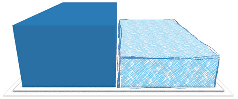
\includegraphics[width=96pt]{prestudy-example-small}
	\vspace{-2.0\baselineskip}
\end{wrapfigure}
Then, images of two blocks, one reference non-sketchy block (left) with a constant height of 100 height units (\emph{\unit{}{hu}}) and the other (right) faced with the study conditions, were shown.
The users were asked to estimate the height of the block on the right.
The input was restricted to a height range of 1 to 200.
During the study, the conditions of the actual block's height, the point of view's angle with a constant distance to the treemap center, and the rendering style varied.

\textbf{Design.}
The experiment was a 3 $\times$ 4 $\times$ 4 mixed design.
Two independent variables, angle and actual height, were tested within-subjects, while the rendering styles were tested between-subjects as follows: 
\textsl{Angle} (0$^\circ$, 15$^\circ$, 30$^\circ$), \textsl{ItemHeight} (36, 77, 132, 187), and \textsl{Style} (Solid, Biro, Pencil, Marker). 
The conditions were fully randomized for each user to prevent order and learning effects.
Aside from training, the number of estimations was 50 participants $\times $ 3 angles $ \times $ 4 heights $ = $ 600.
Each estimation results in an absolute error of the estimated height $\mathit{AbsErr} = |\mathit{ItemHeight} - \mathit{EstimatedHeight}|$, log-transformed for better readability via $\log_2(1+\mathit{AbsErr})$.

\begin{figure}[b!]
	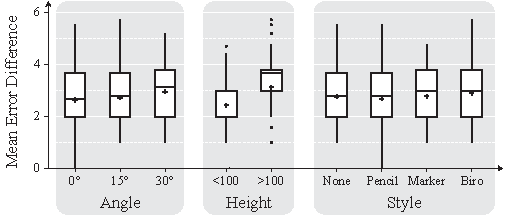
\includegraphics[width=\linewidth]{results-prestudy}
	\caption{Pre-study results depicting the mean error differences for (f.l.t.r.) angle, height, and style groups.}
	\label{fig:results-prestudy}
\end{figure}

\textbf{Results.}
We declared items as unacceptable outliers, if the estimated height was above \unit {100}{hu} as the actual block's height was below \unit{100}{hu} and vice versa.
With this constraint 5 estimates (0.01\%) were removed from the overall trials.
As expected, changing the camera angle results in significant differences (\autoref{fig:results-prestudy}, Angle) in the estimation error ($\mathit{F}_{2,76} = 17.19$, $\mathit{p} < .0001$). 
A post-hoc comparison showed that the angles 0$^\circ$ and 15$^\circ$ yield lower errors by 12\% ($\mathit{p} < .0001$) and 8\% ($\mathit{p} = .003$) respectively compared to an angle of 30$^\circ$.
The error rates \wrt the actual block heights showed significant differences: 
$\mathit{F}_{3,115} = 54.52$, $\mathit{p} < .0001$.
Besides the comparison of \unit{36}{hu} and \unit{132}{hu} ($\mathit{p} = .999$) all differences between pairs were statistically significant in a post-hoc test (all $\mathit{p} < .001$). 
In addition to looking at the four different sampled heights, we split the heights into two groups, one lower and one higher than \unit{100}{hu}.
A one-factorial Anova showed significant differences between these groups:
$\mathit{F}_{1,49} = 72.59$, $\mathit{p} < .0001$ (\autoref{fig:results-prestudy}, Height).
For the varying rendering techniques no significant difference for the height estimation errors was found: $\mathit{F}_{3,43} = .80$, $\mathit{p} < .50$ (\autoref{fig:results-prestudy}, Style).

\subsection{Pre-Attentive Processing (Study I)}
\label{sec:study-preattentive}

\noindent 
Since Biro had a bad performance in early tests---especially under the assumption of equality, \ie all elements having outlines---we focused on Marker and Pencil for pre-attentive perception and, in addition, differentiated between low and high sketchiness (\autoref{fig:order}, 1 and 3).

\textbf{Participants.}
This experiment was conducted with 24 participants (4 female, 20 male) aged 20 to 33 ($\mathit{M} = 24.9$, $\mathit{SD} = 3.4$) and having diverse background knowledge in the field of 2.5D treemaps and visualization in general.

\textbf{Procedure.}
Every participant had to perform 3 tasks (color, sketchiness, conjunction) for a specific rendering style (Marker or Pencil).
We used an eye-tracking setup to ensure that participants had to focus on a fixation cross for a
\begin{wrapfigure}{l}{88pt}
	\vspace{-0.2\baselineskip}
	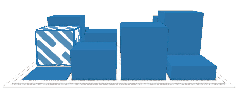
\includegraphics[width=96pt]{study1-example}
	\vspace{-2.0\baselineskip}
\end{wrapfigure}
time of \unit{700}{ms} before an image with the used visual variable was shown for maximum \unit{200}{ms} with a stimulus present or absent.
After each image, users were asked whether they recognized an element that was distinct from all others in color, sketchiness, or a conjunction of both.

\textbf{Apparatus.}
We used an eye-tracking device (EyeFollower\footnote{http://www.interactive-minds.com/eye-tracker/eyefollower} by InteractiveMinds) that allows for accurate gaze-tracking within natural head movements at a desktop environment. 
The participant was placed about \unit{60}{cm} away from a \unit{24}{inch} monitor with a FullHD screen resolution (1080p). 
Additionally, an observation monitor was placed behind a partition wall that allowed the observer to check for losses of head-tracking during the experiment.
The used software recorded gaze sample data at \unit{120}{Hz}. 

\textbf{Design.}
The experiment was a $3 \times 2 \times 2 \times 2$ mixed design with three independent variables (size, presence, sketchiness value) tested within-subjects, while the rendering styles were tested between-subjects:
\textsl{Size} (4 $\times$ 4, 7 $\times$ 7, 10 $\times$ 10), 
\textsl{Presence} (absent, present), 
\textsl{Sketchiness} (low, high),
and rendering \textsl{Style} (Pencil, Marker).
The trials started with the color task, followed by the sketchiness part and the conjunction of both.
Again, we fully randomized the variables tested within-subjects to prevent order and learning effects for \textsl{Size}, \textsl{Presence}, and \textsl{Sketchiness} for each user. 
All in all, 1728 images were shown for 24 (participants) $\times$ 3 (sizes) $\times$ 2 (present/absent) $\times$ 2 (sketchiness values) $\times$ 3 (positions) $\times$ 3 (tasks, color/sketchiness/conjunction).

\begin{figure}[b!]
	\centering
	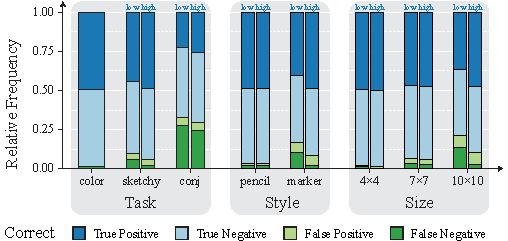
\includegraphics[width=\linewidth]{results-preattentive-study2.pdf}
	\caption{Results of Study I depicting the relative frequency for task, style, and size (low and high sketchiness).}
	\label{fig:results-study1}
\end{figure}

\textbf{Results.}
The results discussed are listed in \autoref{tab:study1-results} and shown in detail in \autoref{fig:results-study1}.
The pre-attentive processing of the visual variable color that serves as a comparative measure for our results showed a very high accuracy as well as precision and recall.
While the trials from the task of pre-attentively processing the implemented sketchiness styles also scored high values, as expected, the conjunction of both performed poorly.
Fisher's exact test significantly showed the independence by tasks ($\mathit{p}<.0005$ for I.TB, I.TS, and I.TC).
A comparison of high and low \textsl{Sketchiness} showed significant differences ($\mathit{p}=.007$ for I.SL and I.SH) with a better accuracy for high sketchiness.
Looking at the different styles, we found a significant difference in the sketchiness task ($\mathit{p}=.0002$ for I.SP and I.SM) with Pencil outperforming Marker in accuracy.
Furthermore, a significant difference between the used sizes ($\mathit{p}<.0001$ for I.S4 and I.SX) was found:
the participants' ability of pre-attentively processing sketchiness decreases as the number of elements increases.

\begin{table}[h!]%
	\caption{Results for pre-attentive processing (Study I).}
	\vspace{-0.5\baselineskip}
	\renewcommand{\arraystretch}{1.618}
	\label{tab:study1-results}
	\centering
	\small
	\begin{tabular}{lrl|lll}
		\# & \bfseries Variable & \bfseries Value & $\mathit{AC}$ & $\mathit{PC}$ & $\mathit{RC}$ \\
		\hline\hline
		I.TB 	& \textsl{Task}			& color/baseline 	& $.991$ & $.995$ & $.986$ \\
		I.TS 	& \textsl{Task}			& sketchiness 		& $.927$ & $.959$ & $.931$ \\
		I.TC 	& \textsl{Task}			& conjunction 		& $.620$ & $.904$ & $.481$ \\
		I.SL 	& \textsl{Sketchiness}	& low 				& $.905$ & $.919$ & $.889$ \\
		I.SH 	& \textsl{Sketchiness}	& high 				& $.947$ & $.925$ & $.972$ \\
		I.SP 	& \textsl{Style}		& pencil 			& $.927$ & $.986$ & $.972$ \\
		I.SM 	& \textsl{Style} 		& marker 			& $.883$ & $.932$ & $.889$ \\
		I.S4	& \textsl{Size} 		& 4 $\times$ 4		& $.991$ & $.993$ & $.993$ \\
		I.S7	& \textsl{Size} 		& 7 $\times$ 7		& $.965$ & $.951$ & $.944$ \\
		I.SX 	& \textsl{Size}			& 10 $\times$ 10 	& $.847$ & $.917$ & $.847$
	\end{tabular}
	
\end{table}

\subsection{Order of Elements (Study II)}
\label{sec:order}

\noindent
Boukhelifa et al. stated that the number of distinct levels for a sketchy rendering style is about 3 to 4 \cite{Boukhelifa2012}.
We implemented these distinct levels for all styles and conducted another study on the ability of participants to bring these levels into correct order (based on the sketchiness value).
The study was again performed as an online survey with 116 participants of whom 91 gave complete answers.

\textbf{Procedure and Design.}
Each survey included 6 sets of 5 images: an image depicting a distinct sketchiness value from non-sketchy to fully sketchy (see \autoref{fig:order}) for each of the three sketchy rendering styles of two different sizes.
The experiment was a 2 $ \times $ 3 within-subject design: 
\textsl{Size} (\emph{coarse}: 3 $ \times $ 3, \emph{fine}: 9 $ \times $ 9)
and rendering \textsl{Style} (pencil, marker). 
The number of images shown was for 91 participants $ \times $ 2 sizes $ \times $ 3 sketchy rendering styles $ = $ 546 tests.

\textbf{Results.}
For each set, a score was calculated (based on the order) representing the number of correctly answered positions, with a range from 0 (all positions wrong) to 5 (completely correct). 
A Kruskal-Wallis test showed significant differences between the rendering styles performance ($\mathit{p} < .001$, \autoref{fig:results-study2}).
A post-hoc comparison showed significant differences between Biro and Marker ($\mathit{p} = .00032$) as well as Biro and Pencil ($\mathit{p} = .00015$). 
However, we could not find this effect in the comparison between Pencil and Marker ($\mathit{p} = .72$).
The Biro style also achieved the highest score ($\mathit{M} = 4.00$, $\mathit{SD} = 1.66$), while Marker ($\mathit{M} = 3.32$, $\mathit{SD} = 1.82$) and Pencil ($\mathit{M} = 3.26$, $\mathit{SD} = 1.79$) achieved similar lower scores. 
Also, we could not find a significant difference between different sizes of images ($\mathit{p} < .001$). 

\begin{figure}[t!]
	\centering
	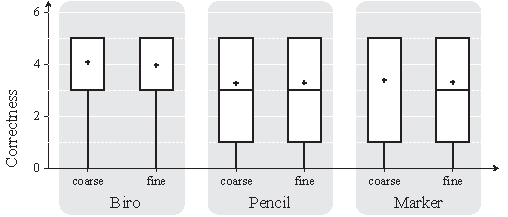
\includegraphics[width=\linewidth]{results-study2}
	\caption{Study II results depicting correctness for (f.l.t.r.) Biro, Pencil, and Marker, each in coarse and fine variation.}
	\label{fig:results-study2}
\end{figure}

